\begin{table}[htbp]\centering\small
\setlength{\tabcolsep}{4pt}
\caption{Paired Gaussian IID null audit. Each procedure uses the same 1,000 datasets in a cell; 499 row draws are nested in 1,999. FWER equals input undercoverage in this all-ties population. Intervals are individual Wilson Monte Carlo intervals.}\label{tab:audit}
\begin{lrbox}{\resultsbox}\begin{tabular}{llrr}
\toprule
$p$, $n$ & Calibration, studentizer, $B$ & FWER & 95\% MC interval\\
\midrule
12, 252 & Row, bootstrap SD, 499 & 0.098 & [0.081, 0.118]\\
12, 252 & Row, bootstrap SD, 1999 & 0.088 & [0.072, 0.107]\\
12, 252 & Row, influence SD, 1999 & 0.085 & [0.069, 0.104]\\
12, 252 & Gaussian, influence SD, 1999 & 0.097 & [0.080, 0.117]\\
52, 252 & Row, bootstrap SD, 499 & 0.215 & [0.191, 0.242]\\
52, 252 & Row, bootstrap SD, 1999 & 0.162 & [0.140, 0.186]\\
52, 252 & Row, influence SD, 1999 & 0.152 & [0.131, 0.176]\\
52, 252 & Gaussian, influence SD, 1999 & 0.188 & [0.165, 0.213]\\
52, 1008 & Row, bootstrap SD, 499 & 0.107 & [0.089, 0.128]\\
52, 1008 & Row, bootstrap SD, 1999 & 0.086 & [0.070, 0.105]\\
52, 1008 & Row, influence SD, 1999 & 0.067 & [0.053, 0.084]\\
52, 1008 & Gaussian, influence SD, 1999 & 0.076 & [0.061, 0.094]\\
\bottomrule\end{tabular}\end{lrbox}\ifdim\wd\resultsbox>\linewidth\resizebox{\linewidth}{!}{\usebox{\resultsbox}}\else\usebox{\resultsbox}\fi\end{table}
At $p=52,n=1008$, the paired FWER difference (499 minus 1,999 row draws with the original studentizer) is 0.021, with Monte Carlo interval [0.007,0.035] based on paired replication differences. The studentizer and mechanism comparisons in Table~\ref{tab:audit} provide separate diagnostics. The verified resampling identities support implementation correctness; the calibration results concern the particular finite-sample procedures.
\begin{figure}[htbp]\centering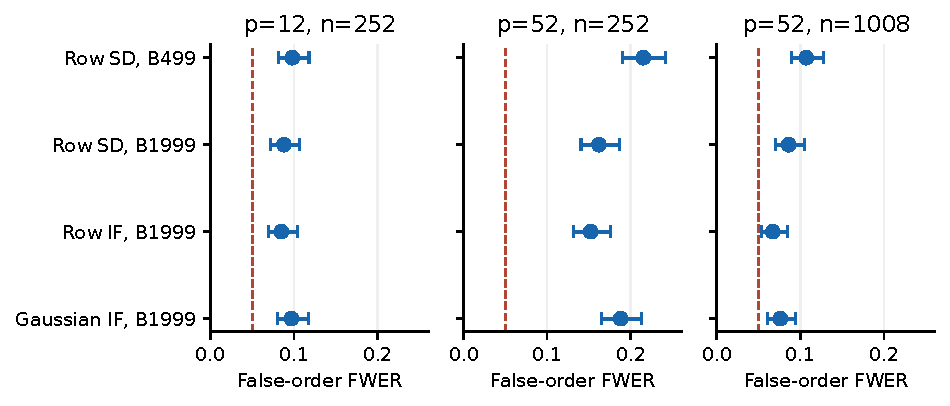
\includegraphics[width=\textwidth]{Fig_audit.pdf}
\caption{False-order FWER in the paired IID audit. Horizontal intervals are individual Wilson Monte Carlo intervals; the vertical line marks 0.05.}\label{fig:audit}\end{figure}
